\chapter{Introduction}\label{CH1}

 
%% Introduce the problem and what we have to overcome to do it
%% last part need to detail all the things that is going in the dissertation nontechnical overview. 



\section{Exoplanets and the Habitable Zone}

 It is amazing that we have observed millions of objects in the universe, but have only detected a few thousand exoplanets. Exoplanets are planets in other star systems and as of February $24^{th}$, 2021 (the date the author started writing her dissertation!) there are 4,352 planets registered on the NASA exoplanet archive \citep{akeson2013nasa}. To put this into context we can compare the number of known exoplanets to other astronomical objects. In a recent Gaia survey, 1.3 million binary stars were cataloged by \cite{el2101million} The SIMBAD database currently details over 12 million objects varying from stars, galaxies, nebulae, supernovae, and more \citep{wenger2000simbad}. From the comparatively limited sample of exoplanet detections, we have discovered that other planetary systems look completely different from our own. The first exoplanet discovered around a sun-like star is 51 Pegasi b, a Jupiter-sized planet that has an orbit closer than Mercury's to its star \citep{mayor1995jupiter}. 

 Astronomers classify exoplanets in reference to our solar system. The categories are based upon exoplanet characteristics such as mass, radius, composition, and semi-major axis of the orbit. These classifications include but are not limited to: hot and cold Jupiters, Neptunes, terrestrial planets, and super-Earths. Figure \ref{fig:massVsemi} plots the known exoplanets as a function of mass and semi-major axis of the orbit \citep{akeson2013nasa}. The mass is in units of Jupiter mass, and the semi-major axis is in units of AU. Almost all of the known exoplanets are larger than Earth, in the Neptune and Jupiter classes. This does not mean that Earth-like planets are rare, but that our current techniques of exoplanet detection are biased.

\begin{figure}
    \centering
    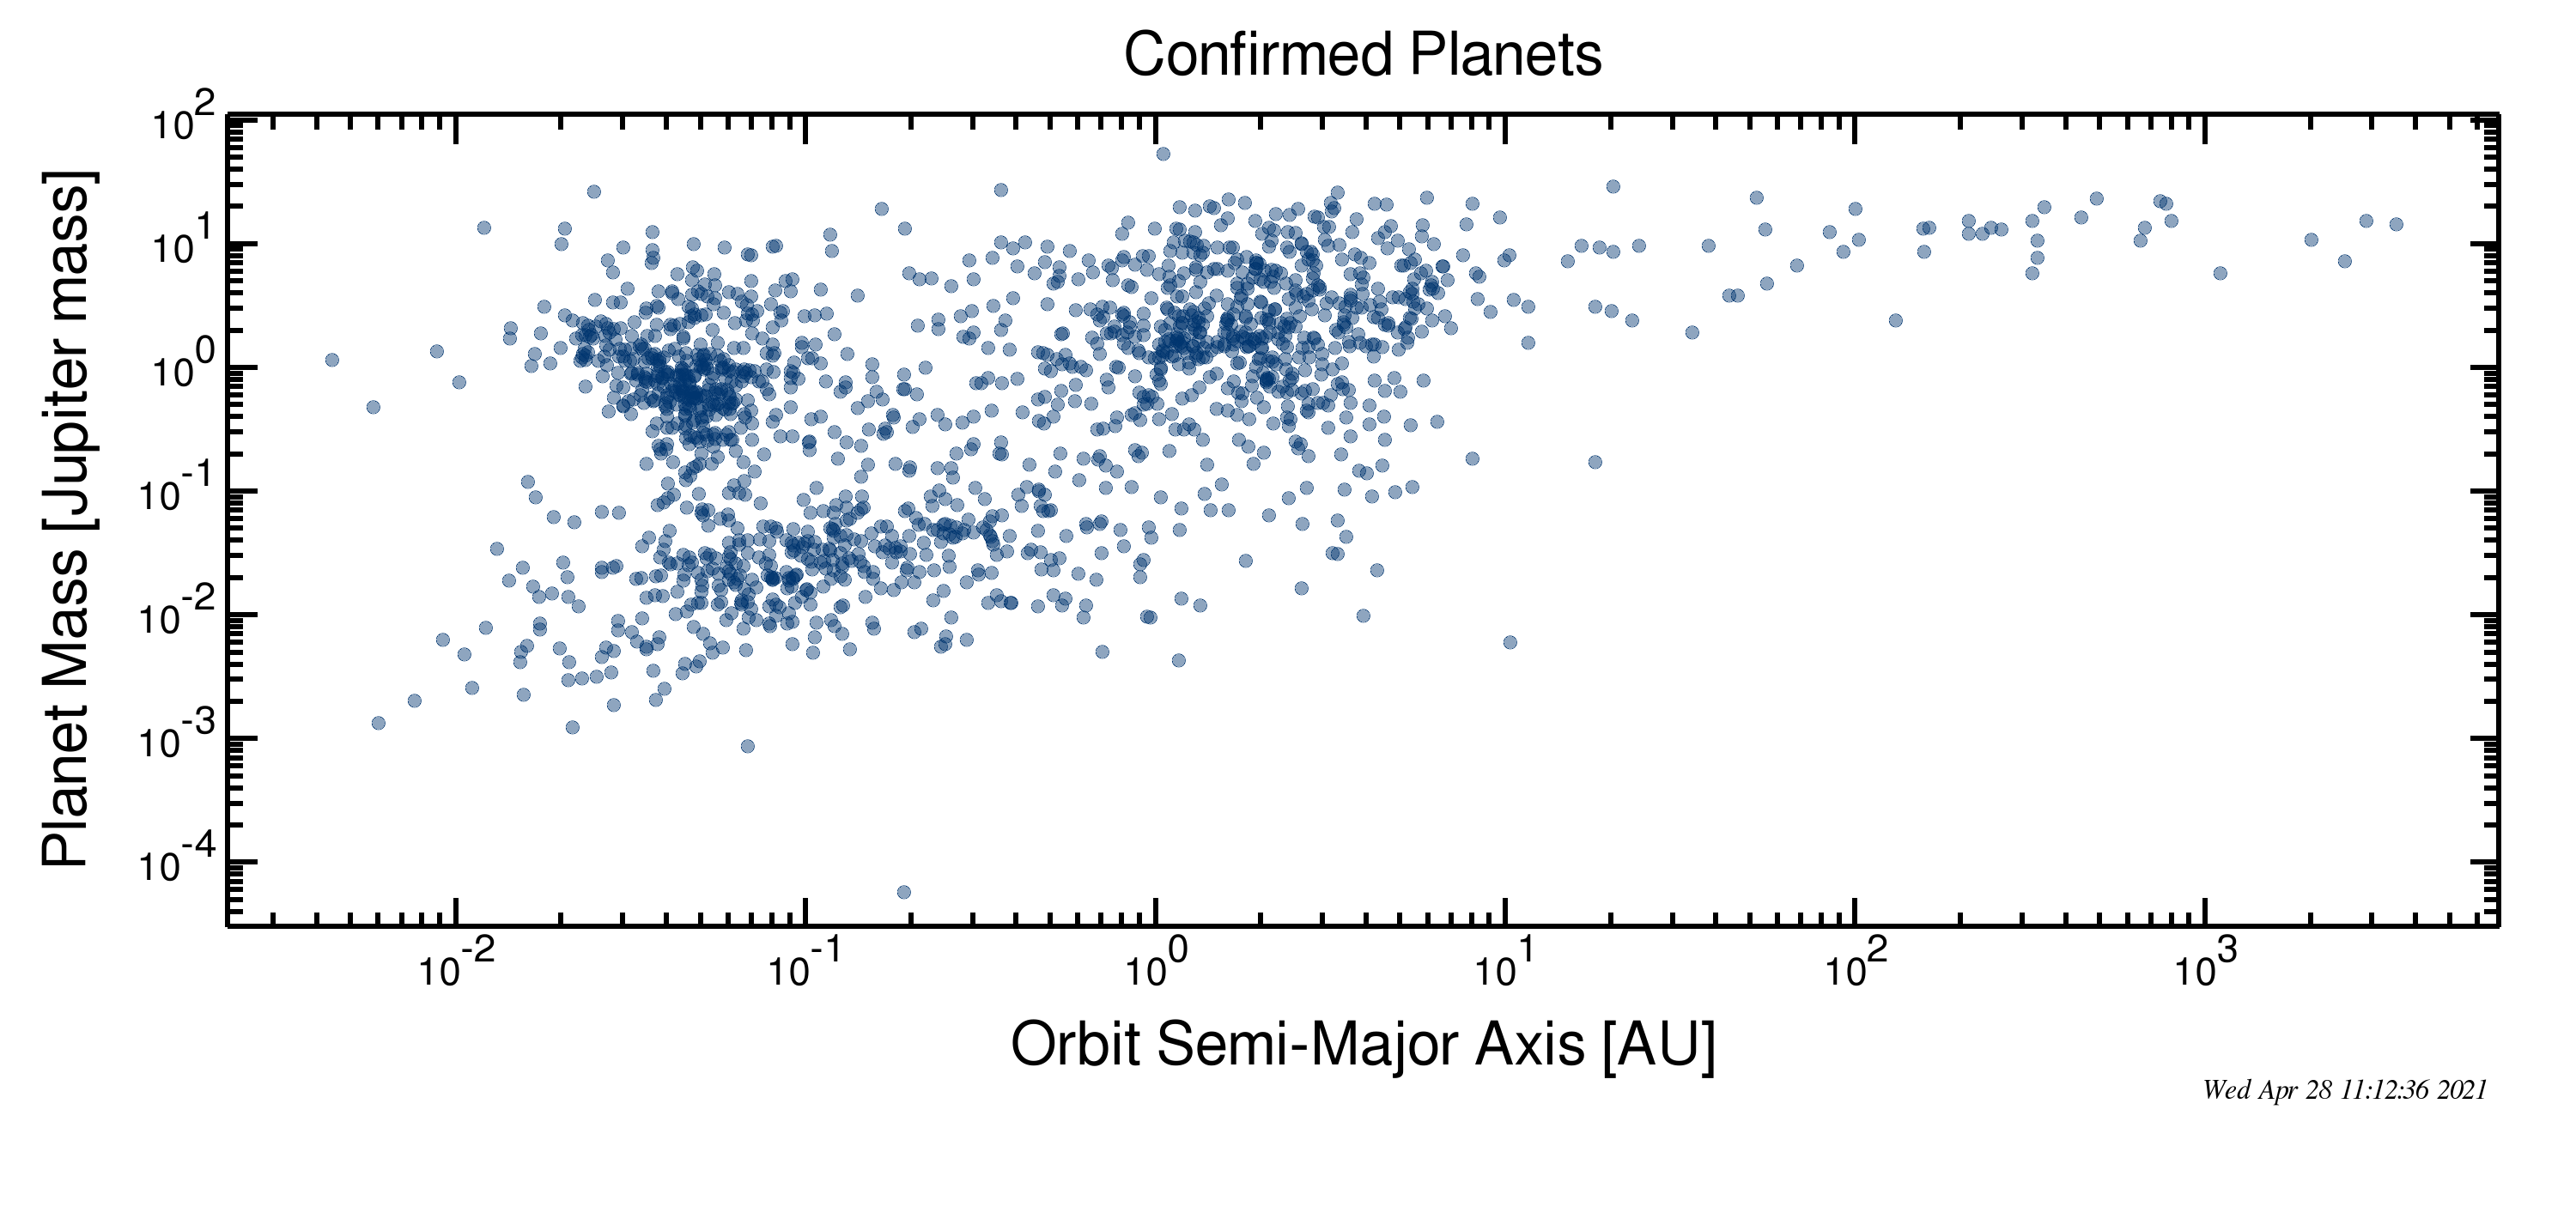
\includegraphics[width=0.8\textwidth]{Chapter Materials/Introduction Materials/MassVsSemiAxis.png}
    \caption{Plot of known exoplanets as a function of mass and semi-major axis. The plot was generated using tools and data provided by the NASA exoplanet archive.}
    \label{fig:massVsemi}
\end{figure}

Two of the driving forces in exoplanet research are the detection and characterization of exoplanets. Different detection techniques favor different types of exoplanets and measure different characteristics. Studying these planetary systems can offer insight into the formation and evolution of our solar system. Of particular interest is the study of Earth-like planets orbiting in a region called the habitable zone. The habitable zone is defined as the region around a star where a terrestrial planet could support liquid water. The bounds of the habitable zone are determined by extremes. The inner edge is defined by the temperature where water escapes from the atmosphere due to a process called photolysis, the decomposition of molecules by light. The outer edge is defined by the formation of carbon monoxide clouds in the atmosphere \citep{seager2010exoplanets}. For our solar system, the Habitable zone is at 0.95-1.37AU. An estimate of the radius of the habitable zone can be found using equation \ref{HabitableZone}, where $L_{\odot}$ is the solar luminosity and $L_{\star}$ is the luminosity of the star \citep{males2014direct}.



\begin{equation}
    a_{HZ} \approx \sqrt{\frac{L_\star}{L_{\odot}}}AU
    \label{HabitableZone}
\end{equation}



\section{Direct Imaging of Exoplanets}

 To study objects close to stars astronomers use a technique called direct imaging. In this method the exoplanet is resolved spatially from the star, allowing for a direct image of the planet to be taken as shown in Figure \ref{fig:exoplanets} \citep{bailey2013hd}. Direct imaging with astrometric calibration allows an astronomer to make precise measurements of the exoplanet’s period, and orbit \citep{seager2010exoplanets}. Using a series of narrowband filters we can measure the flux of the object at different wavelengths. This spectro-photometric characterization allows us to fit models of simulated atmospheres to estimate the composition and structure of the atmosphere \citep{morzinski2015magellan}. This includes features such as clouds and seasons \citep{skemer2012first}. In combination with a spectrograph, we can start to directly characterize the composition of the exoplanet atmosphere by examining emission and absorption lines. 
 

\begin{figure}
    \centering
    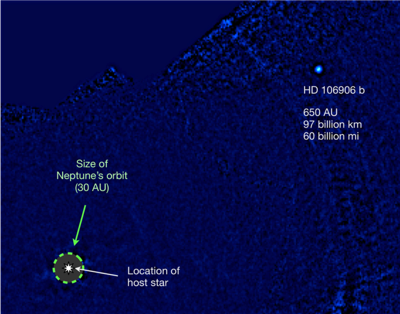
\includegraphics{Chapter Materials/Introduction Materials/Introduction Figures/HCexoplanet.png}
    \caption{Image of exoplanet HD 106906 b taken with the Magellan Adaptive Optics (MagAO) instrument. \citep{bailey2013hd}}
    \label{fig:exoplanets}
\end{figure}



\subsection{High Contrast Imaging}

High contrast imaging is a special case of direct imaging that is used to image faint companions next to bright stars. Targets include circumstellar disks \citep{rodigas2014morphology}, active galactic nuclei \citep{imanishi2020subaru}, and exoplanets \citep{bowler2016imaging}.Typically, exoplanets have flux contrasts of 10$^{-4}$ to 10$^{-10}$ with respect to their host stars. These high contrast ratios present challenges in directly imaging faint objects. Overcoming this contrast problem requires a two-fold solution. The starlight needs to be suppressed by a coronagraph, and the resulting high contrast region, called the dark hole, needs to be maintained over the course of the observation through extreme adaptive optics (ExAO) and wavefront sensing and control (WS$\&$C) techniques. ExAO systems operate by propagating light from a guide star to a wavefront sensor, which measures the phase error of the starlight wavefront. A computer then sends commands to shape a deformable mirror (DM) to correct for the phase error, forming a closed feedback loop that compensates for most of the atmospheric distortion. The corrected beam is then passed to a coronagraph which blocks the light from the on-axis star and allows us to detect faint off-axis sources. Figure \ref{fig:BetaCen} is a high contrast image of the binary star system $\beta$ Centauri using a vector apodizing phase plate coronagraph (vAPP) \citep{snik2012vector}, on the Magellan Adaptive Optics System (MagAO) \citep{close2018status}. There are many types of coronagraphs currently used in high contrast imaging; most work by blocking out light using masks and stops \citep{soummer2004apodized}, or using interferometric techniques to destructively interfere light at the focal plane \citep{foo2005optical}. Uncorrected phase errors and non-common path errors from the ExAO system result in speckles in the focal plane that reduce coronagraph contrast.
 

\begin{figure}
    \centering
    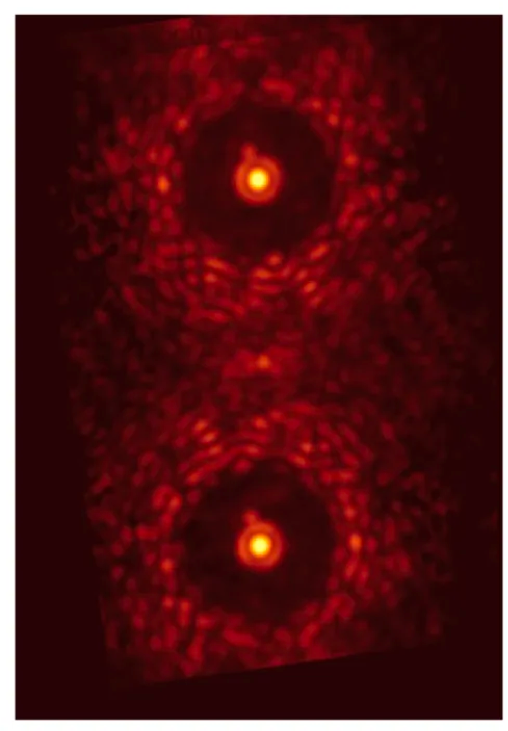
\includegraphics{Chapter Materials/Introduction Materials/BetaCen.png}
    \caption{High contrast image of star system $\beta$ Centauri using a vAPP coronagraph on MagAO. The vAPP creates two copies of the corongraph PSF in a single image. }
    \label{fig:BetaCen}
\end{figure}



\section{Exoplanet Imaging with Giant Segmented Mirror Telescopes}

Within the next decade, the world will see a new generation of Giant Segmented Mirror Telescopes (GSMTs). The Giant Magellan Telescope (GMT) under construction at Las Campanas Observatory, Chile, will have seven 8.4-meter mirrors, forming a 24.5-meter primary mirror \citep{fanson2020overview}. The Thirty Meter Telescope (TMT), and the European Extremely Large Telescope(E-ELT) at Cerro Paranal, Chile, have highly segmented primary mirrors \citep{chisholm2020thirty}. The 39-meter E-ELT primary mirror will be comprised of hundreds of 1.4-meter hexagonal segments \citep{ramsay2020eso}. The TMT will have 492, 1.44-meter hexagonal segments to form the 30-meter primary mirror \citep{sanders2013thirty}. The GSMTs will have the light-collecting power to detect and characterize potentially habitable terrestrial exoplanets for the first time. This will only be achievable if the performance of GSMT-ExAO systems is optimized. Alternative architectures of wavefront sensors are under consideration for GSMT-ExAO instruments considering the trade-offs between detector size, speed, and noise that determine the performance of GSMT-ExAO wavefront control. 

 The GSMTs all plan to use the pyramid wavefront sensor (PWFS) in ExAO instruments. The PWFS performs a Foucault test in two dimensions. Light from the telescope is focused onto a glass pyramid tip where it is split and then the pupil plane is re-imaged onto a detector. The result is copies of the telescope pupil that contain intensity fluctuations that are related to the wavefront phase. All current PWFS on telescopes use a four sided pyramid (4PWFS), resulting in four pupil images. The Planetary Systems Imager \citep{fitzgerald2019planetary}, for the TMT will use a non-modulated PWFS in combination with lower order wavefront control to reach and maintain high contrast \citep{guyon2018wavefront}. The Multi-AO Imaging Camera for Deep Observations (MICADO) for the E-ELT is a pathfinder instrument for performing high contrast imaging on GSMTs that uses a PWFS \citep{davies2018micado}. The High Angular Resolution Monolithic Optical and Near-infrared Integral field spectrograph (HARMONI), also for the E-ELT has a PWFS in the single conjugate adaptive optics (SCAO) mode to deliver diffraction limited performance for the E-ELT's core spectroscopic capability \citep{neichel2016adaptive}. The Giant Magellan Extreme Adaptive Optics System (GMagAO-X) is being developed as a first light ExAO instrument for the GMT and will use a PWFS \citep{males2019gmagao}.

This dissertation aims to develop the three-sided pyramid wavefront sensor (3PWFS) as an alternative GSMT-ExAO wavefront sensor. The 3PWFS  uses fewer detector pixels so it is less sensitive to read noise than the 4PWFS. In Chapter \ref{CH2}, we determine the expected signal from a telescope and detail how atmospheric turbulence degrades image quality. Chapter \ref{CH3} describes the pyramid wavefront sensor and a mathematical formalism based on the diffraction theory description of the Foucault knife-edge test that predicts the intensity pattern after the PWFS. Our formalism allows us to calculate the intensity in the pupil images formed by the PWFS in the presence of phase errors corresponding to arbitrary Fourier modes. We use these results to motivate how we process signals from a 3PWFS. We compare the Raw Intensity method which uses the signal in the pupils as is, and derive the Slopes Maps calculation for the 3PWFS which combines the three pupil images of the 3PWFS to obtain the X and Y slopes of the wavefront. We then use the Object Oriented MATLAB Adaptive Optics toolbox (OOMAO) in Chapter \ref{CH4} to simulate an end-to-end model of an adaptive optics system using a PWFS with modulation and compare the performance of the 3PWFS to the 4PWFS. In Chapter \ref{CH5} we describe the design and current status of the MagAO-X 4PWFS. In Chapter \ref{CH6} we present the Comprehensive Adaptive Optics and Coronagraph Test Instrument (CACTI), which was designed with the flexibility to support visiting instruments and to be easily re-configurable to perform multiple experiments. We first describe the design of CACTI, review its operation and calibration procedures, and discuss its current status. We then discuss an experiment performed on CACTI with a visiting three-sided pyramid wavefront sensor (3PWFS) to explore an alternative wavefront sensor architecture for GSMT-ExAO. Both a 3PWFS and 4PWFS were integrated into  CACTI to demonstrate the operation of a 3PWFS and compare it to the 4PWFS. We present results from experiments demonstrating the operation of the 3PWFS, and comparisons to the 4PWFS. Finally, in Chapter \ref{CH7}, we discuss the conclusions we can draw from the outcome of these experiments.



% Exoplanet signals are small, and need long exposures to overcome photon noise. Astronomers co-add images to beat down the noise, sometimes data across multiple nights are used in a single exoplanet detection. 

%% Habitable zone
% direct imaging
% high contrast imaging
% this is the problem
% here is our solution

%% Chapter two technical background







%\bibliographystyle{IEEEtranS}  
%\bibliography{ThesisBib}


% The search for life and habitable words beyond our solar system is a driving force of modern astronomy and one of the most captivating questions of our time.